\documentclass[9pt]{ieeeconf}

\usepackage{amsmath}
\usepackage[utf8]{inputenc}
\usepackage{kotex}
\usepackage{cite}
\usepackage{graphicx}


% \hypersetup{
%     colorlinks=true,   
%     urlcolor=blue,
% }

\setcounter{secnumdepth}{4}

\renewcommand{\baselinestretch}{1.3}


\begin{document}

\title{ClusterAttentiveFP 기반 화합물의 쓴맛 예측\\
    \large Predict Bitterness of Compound using ClusterAttentiveFP}

\author{Gunhyeong Kim$^{1}$, Chaewon Kim$^{2}$}
\maketitle
\begin{abstract}
    본 논문에서는 ClusterAttentiveFP를 활용하여 화합물의 쓴맛을 예측하는 모델을 제안한다.
\end{abstract}
\begin{keywords}
    ClusterAttentiveFP, 쓴맛, 화합물, attention machanism
\end{keywords}


\section[short]{\Large {\textsc{Introduction}}}

\indent 동물은 독성 화합물을 섭취하지 않도록 선천적으로 쓴맛에 대하여 혐오감을 느끼도록 진화하였다.
그러므로 약물이 쓴맛을 낼 경우, 환자의 불쾌감을 유발하여 복용 준수성을 저해할 수 있다\cite{dagan2017bitter}.
특히 소아 환자에 대하여 복약 순응도 문제를 유발할 가능성이 크며\cite{bahia2018bitterness},
실제로 소아과 의사의 90\% 이상이 약의 맛이 완치의 가장 큰 장애물이라고 답했다\cite{mennella2013bad}.
더하여, 반려동물 보유 가구 수가 전체 가구 수의 25.7\% 에 달하면서, 반려동물의 약물 치료에 대한 관심이 커지고 있다.
이에 따라 약물의 쓴맛이 반려동물의 복약 용이성에 미치는 영향 또한 연구 대상으로 남아있다.

\indent 그러므로 약물의 쓴맛에 대한 연구는 약물 치료의 효과를 향상하는 데 매우 중요하다.
약물의 쓴맛을 완화할 수 있다면, 소아 환자 또는 반려동물에 대한 복약 지도가 편리해질 것이다.

\indent TAS2R38는 2번 맛 수용체 38호를 결정하는 단백질 생성 유전자이다.
2번 맛 수용체 3호는 입과 소화기관 내에서 쓴맛을 인지하고 구분해내는데, 이 유전자는 인간뿐만 아니라 반려동물로 가장 많이 고려되는 종인 개와 고양이에도 존재한다.
그러므로 사람을 대상으로 충분한 연구가 선행된다면 반려동물로의 확장 또한 가능하리라 생각된다.

\indent 기존의 이러한 연구는 대부분 \textit{in vivo}, \textit{in vitro} 환경에서 진행되어 비용 소모가 컸다.
이를 \textit{in silico} 환경에서 인공지능 모델을 사용하여 예측할 수 있다면 비용 절감 및 실험의 윤리성과 안전성을 확보할 수 있을 것이다.

\section[short]{\Large {\textsc{Materials and Methods}}}
\subsection[short]{\large {Data sets}}
화합물의 맛 정보(단맛, 쓴맛, 짠맛, 신맛, 감칠맛, 무맛 등)가 정리되어 있는 ChemTastesDB\cite{rojas2022chemtastesdb}를 데이터 셋(data set)으로 활용하였다. 쓴맛을 나타내는 화합물을 1, 그 외 단맛, 짠맛, 신맛, 감칠맛, 무맛 등 다섯 가지 미각을 나타내는 화합물을 0으로 라벨링(labeling)하였다.
ChemTastesDB에는 화합물의 맛 정보 이외에도 분자 구조를 문자열로 표기한 canonical SMILES 정보가 존재한다. RDkit이 제공하는 모듈을 활용하여 이 canonical SMILES 표기로부터 먼저 분자 객체(moleculer object)를 추출한 다음, 분자의 구조적 정보와 물리‧화학적 정보를 추출하였다.

\section[short]{\Large {\textsc{Background}}}
\subsection[short]{\large {Graph}}
\indent 그래프란 자료구조의 종류 중 하나로, 정점(node)와 그 정점을 연결하는 간선(edge)으로 구성되어 있다.
그렇기 때문에 연결되어 있는 객체 간의 관계를 표현할 수 있다. 그래프는 이러한 특징을 통해 뇌를 구성하는 뉴런 간의 연결성, 지식 그래프(knowledge graph), 화학 분자, 단백질 상호작용 등을 표현하는 데 적합하다.
그러므로 이러한 그래프를 잘 분석할 수 있다면 신약 개발 등의 생화학적 분야 뿐만 아니라 인공지능 개발 등의 공학 분야에 큰 기여를 할 수 있을 것이다.

\indent 그래프에는 다음과 같은 다양한 특징들이 존재한다. 첫째, 방향(directed)과 양방향(undirected), 둘째, 사이클 혹은 루프가 존재 할 수 있으며 자체 간선(self-roop) 또한 가능하다.
셋째, 루트 정점(root node) 또는 부모-자식 정점의 개념이 존재하지 않는다.

\indent 그래프는 주로 인접행렬(adjacency matrix) 또는 인접리스트(adjacency list)로 표현된다. 정점의 개수가 n개일 때 인접행렬의 크기는 $n \times n$이며, 인접리스트의 크기는 $n$이다. 인접행렬은 정점 간의 연결 관계를 행렬로 표현한 것이다. 인접리스트는 정점의 개수만큼 리스트를 만들고, 각 리스트에는 해당 정점과 연결된 정점들을 저장한다.
\begin{figure}[h]
    \centering
    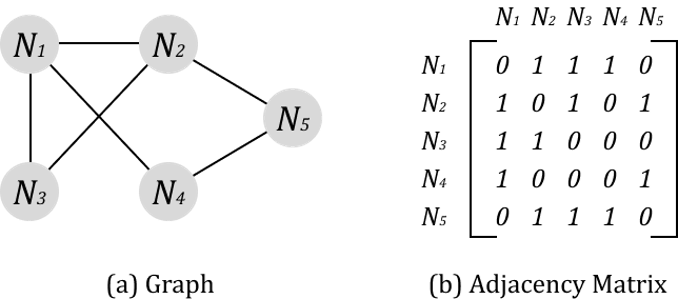
\includegraphics[width=0.5\textwidth]{./images/adjacency_matrix.png}
    \caption{그래프와 인접행렬의 예시}
\end{figure}

\subsection[short]{\large {Node Embedding}}
\indent 정점 임베딩은 그래프의 정점들을 벡터의 형태로 표현하는 것이다. 그래프에서의 위상적 거리를 임베딩한 벡터 공간에서도 보존하는 것을 목표로 한다. 
즉, 가까운 위상적 거리를 가진 정점들은 벡터 공간에서 가깝게, 먼 위상적 거리를 가진 정점들은 벡터 공간에서 멀게끔 임베딩하는 것이다.

\subsection[short]{\large {Graph Neural Network}}
그래프 신경망이란 그래프를 분석하는 AI 기법 중 하나이다. 그래프 신경망 기법에도 여러 가지가 있으나, 
최근 일반적으로 사용되는 기법은 그래프의 인접행렬과 정점들의 특징 행렬(feature matrix)를 활용하는 방식이다. 
인접행렬과 정점의 특징 행렬을 곱한 결과값을 활용하여 정점의 특징 벡터를 업데이트 해 나간다. 
이 과정에도 다양한 기법이 존재하는데, 대표적인 기법이 message-passing 함수이다. 
특정 정점과 연결된 주변 정점들의 정보를 활용하여 정점의 정보를 업데이트하는 과정을 반복하다가, 
분류(classification)과 같은 최종 목표를 위해 전체 그래프의 표현(representation)을 추출하는 방식이다.

\subsection[short]{\large {Multi-Layer Perceptron; MLP}}
\indent 퍼셉트론은 인공 신경망의 기본 단위로, 입력 신호에 가중치(weight)와 편향(bias)을 적용하여 출력 신호를 생성하는 구조이다. 
퍼셉트론은 인간 뇌를 구성하는 뉴런의 구조를 모방한 것이다.

\indent 다층 퍼셉트론은 인공 신경망의 한 종류로, 여러 층의 퍼셉트론(perceptron)을 연결한 신경망이다. 이미지, 텍스트, 음성 등 다양한 데이터를 처리하는 데 활용된다. 
다층 퍼셉트론은 일반적으로 입력층(input layer), 은닉층(hidden layer), 출력층(output layer)으로 구성되어 있다. 
다층 퍼셉트론의 학습에서는 순전파(forward-propagation)와 역전파(back-propagation)가 일어나면서 가중치와 같은 파라미터가 학습되어 입력 값에 대한 적절한 출력 값을 출력할 수 있게 된다.

\subsection[short]{\large {SMILES(Simplified Molecular Input Line Entry System) 표기법}}\
\indent SMILES는 ASCII 문자로 표현된 분자 구조 표현 방식으로 화학 정보를 처리하는 데 사용되는 표준 형식이다. SMILES는 원자, 원자간 결합, 치환기, 고리 등의 다양한 정보를 표현할 수 있다. 
SMILES는 ASCII 문자로 표현되기 때문에 다른 표기법에 비해 간결하고, 다양한 분자를 표현할 수 있다는 장점이 있으나, 동일한 분자에 대해 여러 가지의 SMILES가 존재할 수 있다. 
예를 들어, 에탄올($C_2 H_6 O$)은 C2H5OH, H2C-CH2-OH와 같은 두 가지의 SMILES로 표기될 수 있다. 이러한 한계를 극복하기 위해 canonical SMILES 표기법이 고안됐다.
이 방식은 동일한 분자를 표현하는 단 하나의 SMILES를 제공한다. 이를 위해 canonical SMILES는 다음과 같은 규칙을 사용한다.

\begin{enumerate}
    \item 원자의 순서: 원자 번호 순서로 정렬된다.
    \item 치환기의 순서: 치환기의 종류 순서로 정렬된다.
    \item 결합의 방향: 결합의 방향이 고정된다.
\end{enumerate}

\subsection[short]{\large {Morgan Fingerprint}}
Fingerprint는 분자의 구조적 특징을 나타내는 정수값으로, 분자를 고유하게 식별하고 유사성을 측정하는 데 사용된다. 
또한, 분자 그래프의 정점 특징 벡터로써 사용되기도 한다. 
Fig. 2.와 같이 어떤 목표 원자로부터 일정한 거리에 있는 원자들을 분석하여 식별자를 부여하고,
이 식별자들에 hash function을 적용하여 이진수 값을 얻을 수 있다. 
이때 hash function으로 morgan algorithm을 사용하면 Morgan fingerprint를 얻을 수 있다. 
\begin{figure}[h]
    \centering
    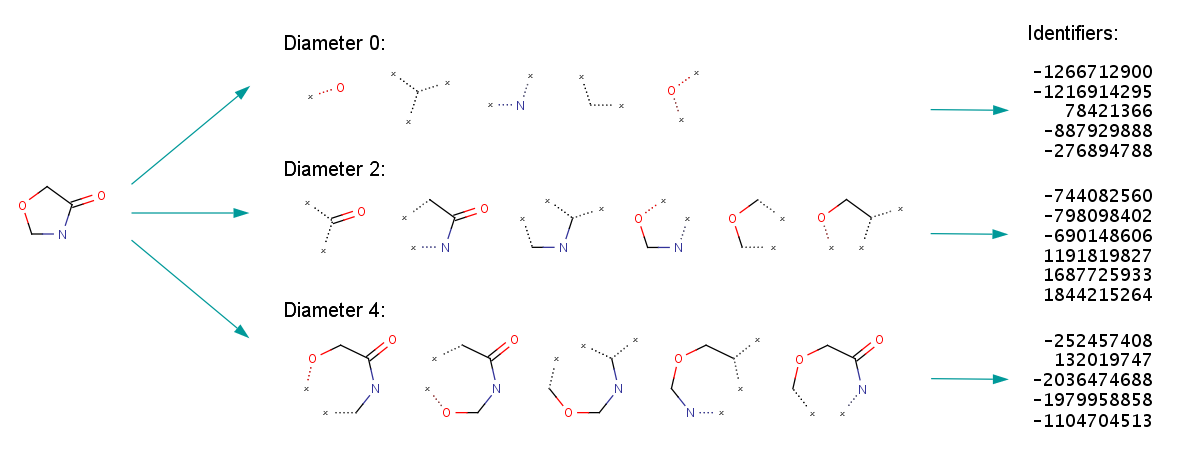
\includegraphics[width=0.5\textwidth]{./images/mf.png}
    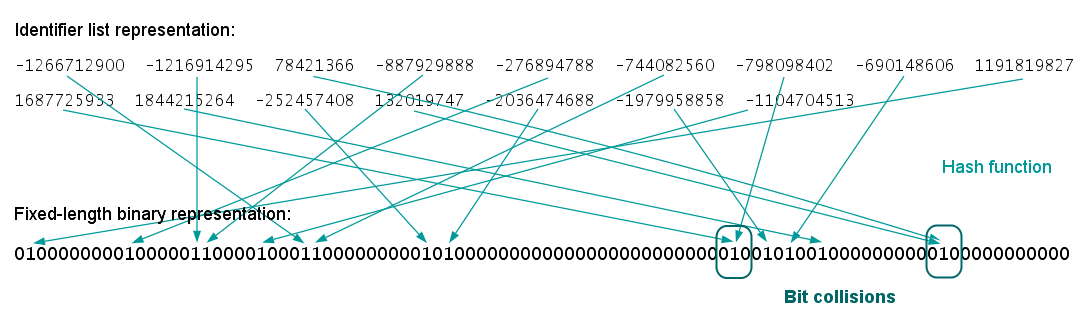
\includegraphics[width=0.5\textwidth]{./images/mf_hash.png}
    \caption{Morgan fingerprint 생성 과정}
\end{figure}

 
% \section[short]{\Large {\textsc{References}}}
\bibliographystyle{IEEEtran}
\bibliography{IEEEabrv, ref}

\end{document}

